\section{Ablauf}\label{sec:ablauf}
Zur Untersuchung der Kommunikation zwischen der Geräten wird der Verkehr auf den LAN-Schnittstellen in verschiedenen Szenarien betrachtet:

\begin{enumerate}
    \item Echo Dot
    \begin{enumerate}[label*=\arabic*.]
        \item Einschalten
        \item 5 Minuten reiner Netzverkehr (keine Befehle)
        \item Erfragen des aktuellen Wetters
    \end{enumerate}
    \item Playstation 4
    \begin{enumerate}[label*=\arabic*.]
        \item Ein- und Ausschalten über \textit{Hassbian}
        \item Ein- und Ausschalten über \textit{Harmony Hub}
    \end{enumerate}
    \item Kodi
    \begin{enumerate}[label*=\arabic*.]
        \item Navigieren mit Pfeiltasten in der Smartphone-App
        \item Kurzes Fernsehen gesteuert von der Smartphone-App
    \end{enumerate}
\end{enumerate}

Eine detaillierte Beschreibung der Szenarien folgt in Kapitel. \todo[inline]{Kapitel hinzufügen}


Alle in den Szenarien betrachteten Verbindungen sind LAN-Verbindungen und werden über den zentralen Router des lokalen Netzwerk transportiert.
Folglich ist dies auch eine nützliche Stelle um den anfallenden Verkehr mitzuschneiden.
In diesem Fall handelt es sich bei dem Router um eine \textit{FRITZ!Box 7560}\cite{FRITZBox29:online}.
Wie auch andere FRITZ!Boxen stellt diese unter der Adresse \url{http://fritz.box/html/capture.html} eine Oberfläche bereit,
um Datenpakete an verschiedenen Schnittstellen mitzuschneiden
und in einem für das bekannte Tool \textit{Wireshark} lesbaren Format herunterzuladen.

\begin{figure}[ht!]
    \centering
    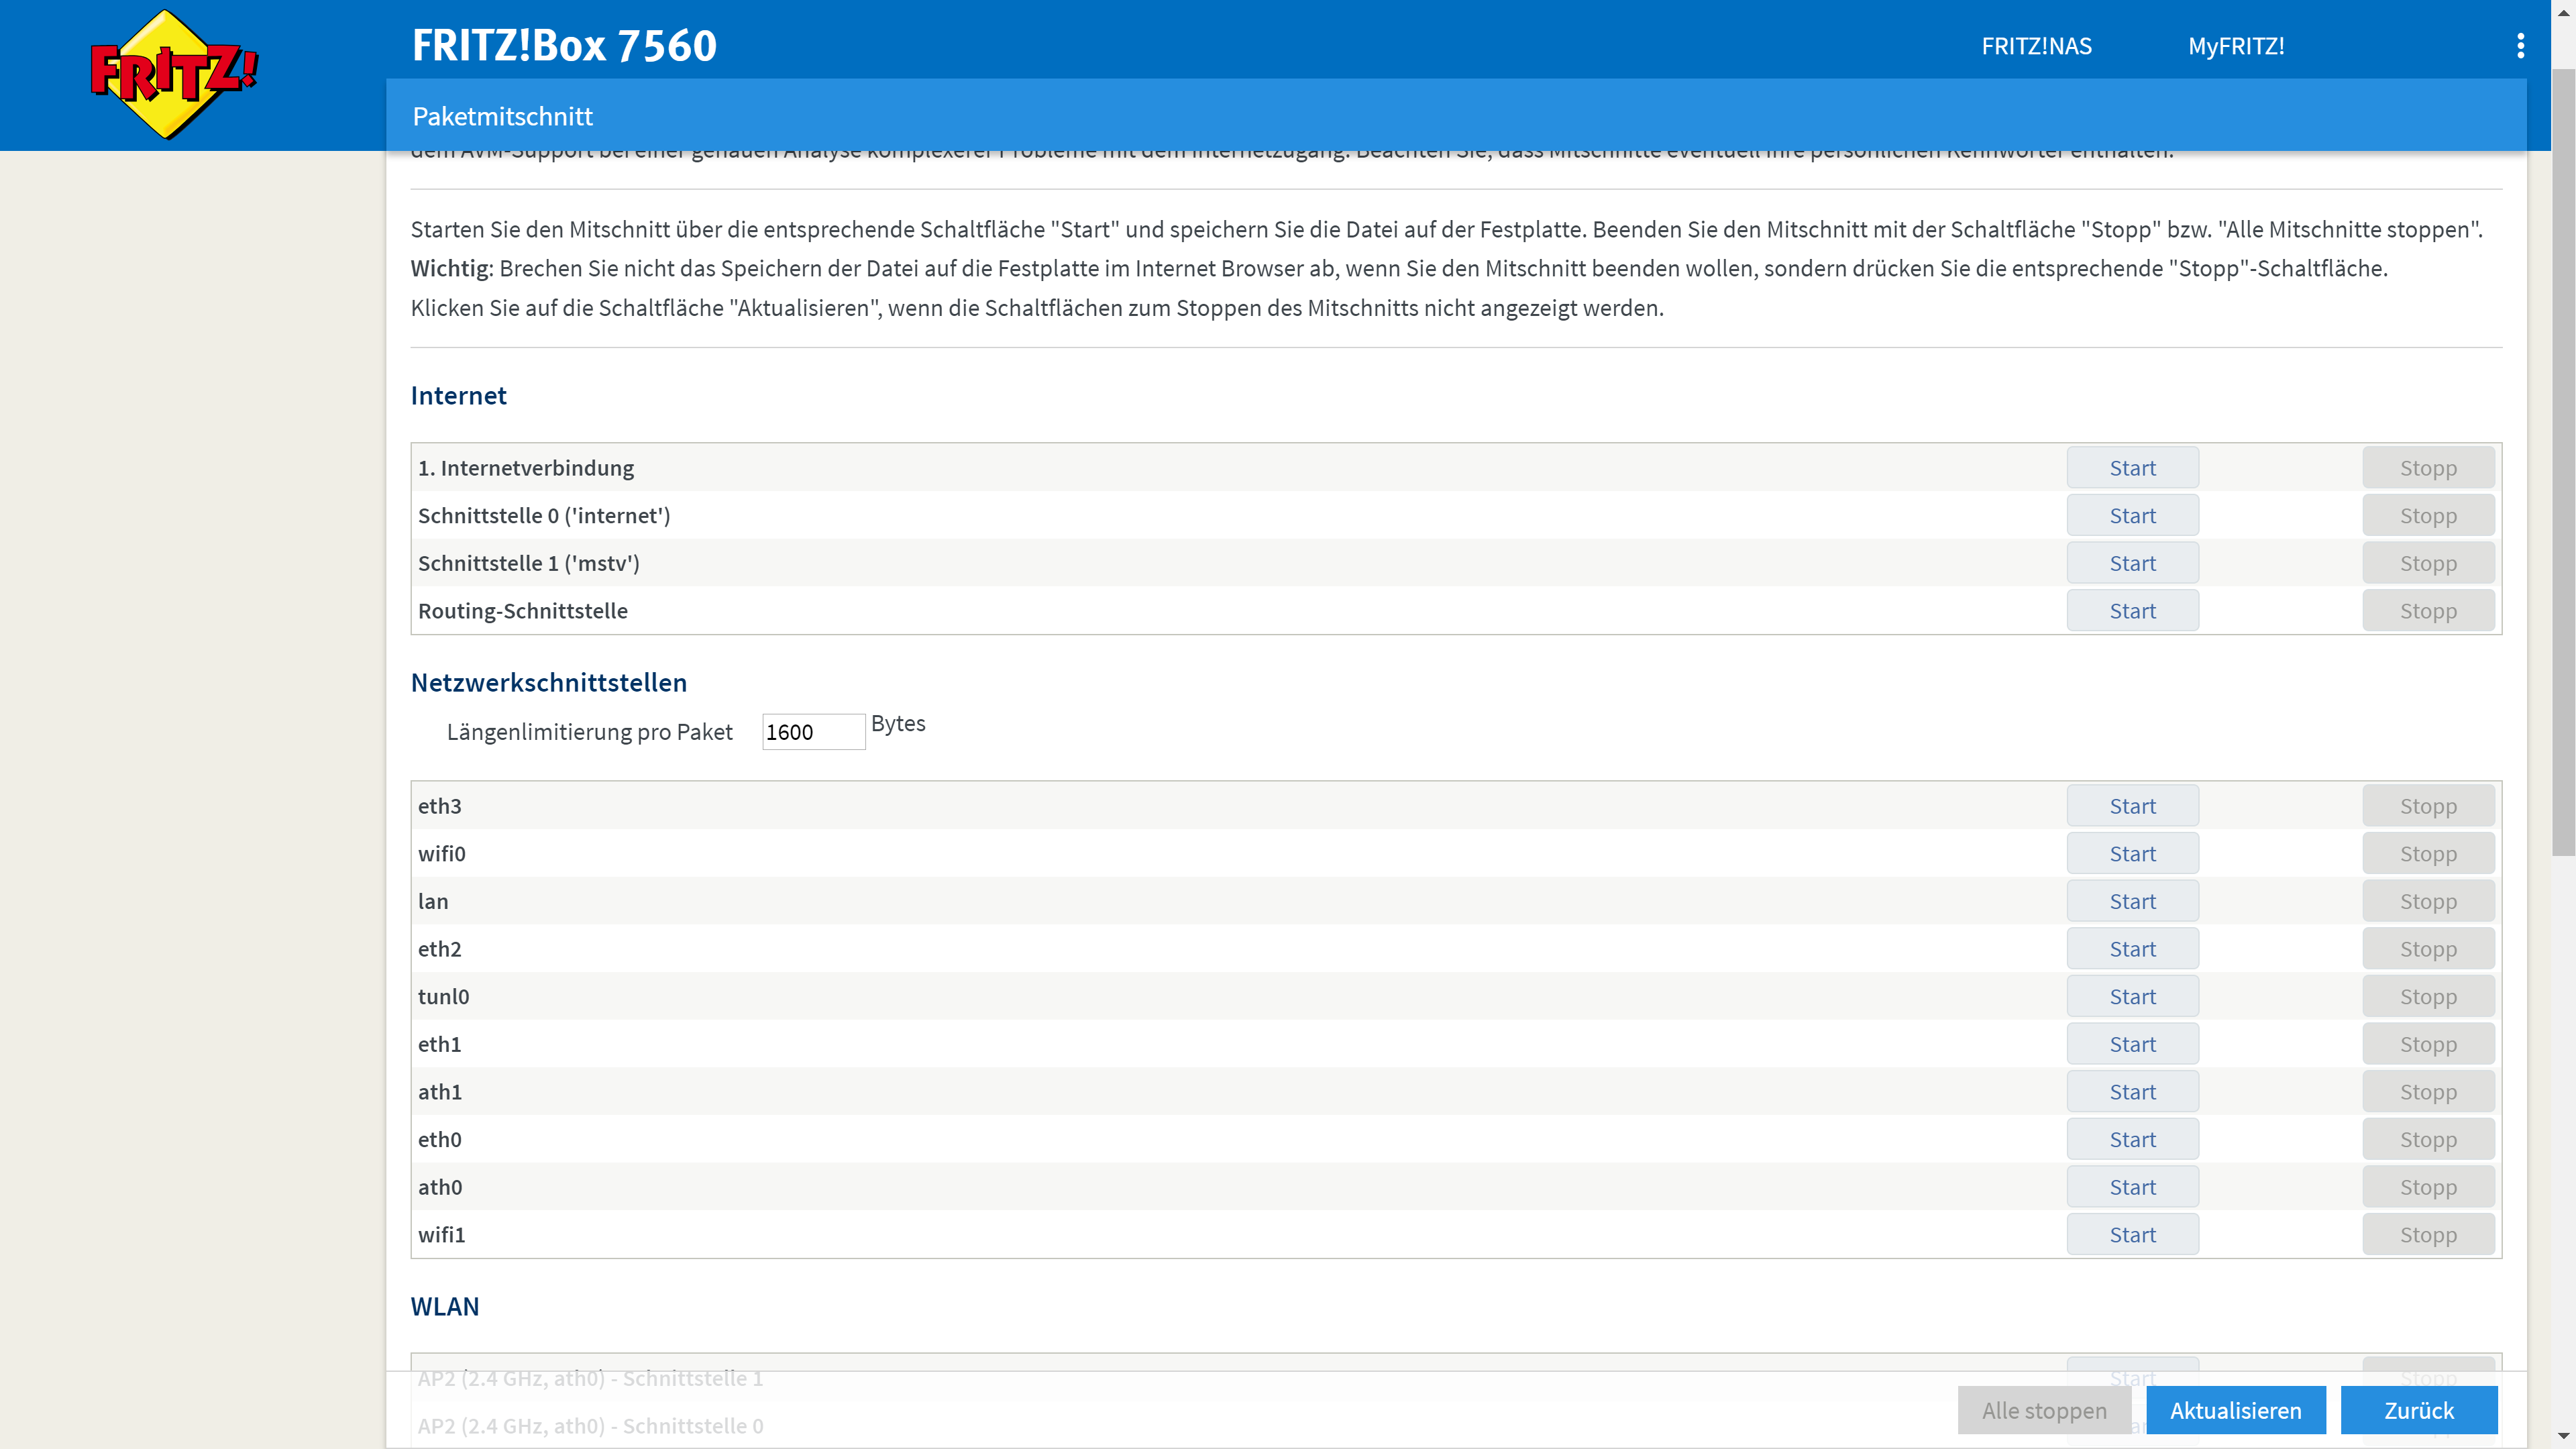
\includegraphics[width=\textwidth]{fribCapture}
    \caption{FRITZ!Box Weboberfläche für Paketmitschnitte}\label{fig:fribCapture}
\end{figure}

Diese Methode bringt zwei entscheidente Vorteile mit sich:
Zum Einen läufte der gesamte Verkehr durch den Router, da alle Geräte per (W)LAN an diesen angeschlossen sind.
Zum Anderen können dort die Pakete unkompliziert mitgeschnitten werden. Zugriff auf die zu betrachtenden Geräte
oder gar ein Umleiten des Verkehrs auf einen Computer, beispielsweise durch \textit{Spoofing}\cite{Maninthe12:online} sind nicht notwendig.

Jedoch hat diese Methode auch einen Nachteil:
Die Oberfläche für Paketmitschnitte ist nicht für den allgemeinen Nutzer,
sondern eigentlich zur Unterstützung des Supports bei kopmplexen Problemen bestimmt.
Daher wird die Seite auch nicht detailliert dokumentiert.
Lediglich eine kurze Anleitung wie solle Paketmitschnitte gestartet und gestoppt werden befindet sich im oberen Bereich der Seite.
Die in \autoref{fig:fribCapture} zu sehenden zahlreichen Schnittstellen werden nicht näher spezifiziert.

In \cite{fritzcap8:online} präsentiert Jeroen Wiert Pluimers die Ergebnisse einer Analyse der Schnittstellen.
Hier hervorzuheben ist die Schnittstelle \texttt{ath0}. Als WLAN-Schnittstelle scheint sie gut für dieses Projekt geeignet zu sein.

Ein rudimentärer praktischer Vergleich mit den Schnittstellen \texttt{lan} und \textit{Routing-Schnittstelle} zeigt,
dass in dem Mitschnitt von \texttt{ath0} alle Pakete der zu betrachtenden Komponenten enthalten sind.

Der Mitschnitt von \texttt{lan} enthält zwar auch alle Pakete der zu betrachtenden Komponenten.
Enthält jedoch auch viele andere Pakete was zu einem erhöhten Overhead führt.

Der Mitschnitt der \textit{Routing-Schnittstelle} enthält lediglich Pakete welche vom Router an das Internet gesendet oder aus diesem Empfangenw werden.
Diese Schnittstelle ist daher für den lokalen Verkehr ungeeignet.


Das Erfassen der Pakete für eines der Szenarion folgt folgendem Muster:
\begin{enumerate}
    \setlength\itemsep{-0.5em}
    \item Starten des Paketmittschnitts auf \texttt{ath0}
    \item Durchführen des Szenarios
    \item Beeenden des Paketmittschnitts
    \item Öffnen des Mitschnitts mit \textit{Wireshark} und filtern der relevanten Pakete
    \item Speichern des gefilterten Mitschnitts zur späteren Analyse
    \item Wiederholen des Vorgangs, um je zwei Mitschnitte pro Szenario zur genaueren Analyse zu erhalten
\end{enumerate}